\documentclass[12pt]{article}%
\usepackage{hyperref}
\usepackage{listings}
\usepackage{color}
\usepackage{multicol}
\usepackage{amsfonts}
\usepackage{fancyhdr}
\usepackage{comment}
\usepackage[a4paper, top=2.2cm, bottom=2.2cm, left=2.2cm, right=2.2cm]%
{geometry}
\usepackage{times}
\usepackage{changepage}
\usepackage{amssymb}
\usepackage{graphicx}%
\newtheorem{theorem}{Theorem}
\newtheorem{acknowledgement}[theorem]{Acknowledgement}
\newtheorem{algorithm}[theorem]{Algorithm}
\newtheorem{axiom}{Axiom}
\newtheorem{case}[theorem]{Case}
\newtheorem{claim}[theorem]{Claim}
\newtheorem{conclusion}[theorem]{Conclusion}
\newtheorem{condition}[theorem]{Condition}
\newtheorem{conjecture}[theorem]{Conjecture}
\newtheorem{corollary}[theorem]{Corollary}
\newtheorem{criterion}[theorem]{Criterion}
\newtheorem{definition}[theorem]{Definition}
\newtheorem{example}[theorem]{Example}
\newtheorem{exercise}[theorem]{Exercise}
\newtheorem{lemma}[theorem]{Lemma}
\newtheorem{notation}[theorem]{Notation}
\newtheorem{problem}[theorem]{Problem}
\newtheorem{proposition}[theorem]{Proposition}
\newtheorem{remark}[theorem]{Remark}
\newtheorem{solution}[theorem]{Solution}
\newtheorem{summary}[theorem]{Summary}
\usepackage{commath}
\usepackage{url} 
\usepackage{hyperref}
\usepackage[style=numeric]{biblatex}
\usepackage{subfig}
\usepackage{minted}
% \usepackage[utf8]{inputenc}
% \usepackage[english]{babel}
\usepackage{esvect}
\addbibresource{reference.bib}


\usepackage{commath}

\newenvironment{proof}[1][Proof]{\textbf{#1.} }{\ \rule{0.5em}{0.5em}}
\usepackage[utf8]{inputenc}

% \usepackage{algorithm}
% \usepackage{algorithmic} %format of the algorithm


% Default fixed font does not support bold face
\DeclareFixedFont{\ttb}{T1}{txtt}{bx}{n}{12} % for bold
\DeclareFixedFont{\ttm}{T1}{txtt}{m}{n}{12}  % for normal

\usepackage{graphics}

% Custom colors
\usepackage{color}
\definecolor{deepblue}{rgb}{0,0,0.5}
\definecolor{deepred}{rgb}{0.6,0,0}
\definecolor{deepgreen}{rgb}{0,0.5,0}

\usepackage{listings}
\newcommand{\Q}{\mathbb{Q}}
\newcommand{\R}{\mathbb{R}}
\newcommand{\C}{\mathbb{C}}
\newcommand{\Z}{\mathbb{Z}}

% Python style for highlighting
\newcommand\pythonstyle{\lstset{
language=Python,
basicstyle=\ttm,
otherkeywords={self},             % Add keywords here
keywordstyle=\ttb\color{deepblue},
emph={MyClass,__init__},          % Custom highlighting
emphstyle=\ttb\color{deepred},    % Custom highlighting style
stringstyle=\color{deepgreen},
frame=tb,                         % Any extra options here
showstringspaces=false            % 
}}

% Python environment
\lstnewenvironment{python}[1][]
{
\pythonstyle
\lstset{#1}
}
{}

% Python for external files
\newcommand\pythonexternal[2][]{{
\pythonstyle
\lstinputlisting[#1]{#2}}}
\usepackage[utf8]{inputenc}
\usepackage{amsmath, nccmath}
\usepackage{geometry}

\usepackage{algorithm}
\usepackage{arevmath}     % For math symbols
\usepackage[noend]{algpseudocode}

\begin{document}

\title{Institute of Robotics,  University of Innopolis}
\author{Computational Intelligence \\ Linear Programming}
\date{\today}
\maketitle

\section{Task 01}

\begin{equation}
\begin{aligned}
\max_{\mathbf{x}} \quad & x_1 + x_2\\
\textrm{s.t.} \quad & 9x_1 + 3x_2 \leq 56,\\
 \quad & -7x_1 + 9x_2 \leq 56,\\
 \quad & -1 \leq \mathbf{x} \leq 1
\end{aligned}
\end{equation}

\begin{enumerate}
    \item Formulate the problem using CVXPY and scipy.optimize.linprog \url{https://docs.scipy.org/doc/scipy/reference/generated/scipy.optimize.linprog.html}
\end{enumerate}


\section{Task 02}

You are given three non empty sets:

\begin{equation*}
\begin{aligned}
x_{(1)},...,x_{(n)} \\
y_{(1)},...,y_{(m)} \\
z_{(1)},...,z_{(p)} \\
\end{aligned}
\end{equation*} in $\mathbb{R}^n$ where you have to find corresponding affine functions in the following form:
\begin{equation}\label{eq:line}
    f_i(\mu) = a_i^T\mu -b_i, \; i=1,2,3, \; \mu = x,y,z
\end{equation} subject to the following constraints:

\begin{equation*}
\begin{aligned}
\quad & f_1(x_{(j)}) > max \{f_2(x_{(j)}), f_3(x_{(j)})\}, \; j = 1,...,n\,\\
  \quad & f_2(y_{(j)}) > max \{f_1(y_{(j)}), f_3(y_{(j)})\}, \; j = 1,...,m\,\\
  \quad & f_3(z_{(j)}) > max \{f_1(z_{(j)}), f_2(z_{(j)})\}, \; j = 1,...,p\,\\
 \quad & a_1 + a_2 + a_3 = 0, \\
 \quad & b_1 + b_2 + b_3 = 0 ,
\end{aligned}
\end{equation*}

\begin{enumerate}
    \item Use the following script for generating three sets in $\mathbf{R}^2$ and solve (\ref{eq:line}) using CVXPY
    
    
\begin{minted}
[frame=lines, framesep=2mm, baselinestretch=1.2,]
{python}

import numpy as np
import cvxpy as cp 
import matplotlib.pyplot as plt 
import random 
from random import random
import math


def get_circle(U):
    cx = cp.Variable()
    cy = cp.Variable()
    obj = cp.Minimize(cp.norm(cp.vstack((U[0,:] - cx, U[1,:] 
        - cy))))
    prob = cp.Problem(obj, [])
    prob.solve()

    cx, cy = map(lambda x: x.value, [cx, cy])
    xc = np.array([cx, cy])
    r_hat = (U.T - xc)
    mean_r = np.sum(r_hat * r_hat, axis=1).mean()
    r = np.sqrt(mean_r)
    return xc, r

def draw_circles(sets):
    ax = plt.gca()
    for set_i in sets:
        xc, r = get_circle(set_i)
        circle = plt.Circle(xc, r, fill=False)
        ax.add_patch(circle)
        
def clusters(n, points, centers, r):
    sets = []
    def cluster(points, center, radius):
        npoints = 50
        r = radius 
        t = np.linspace(0, 2*np.pi, npoints, endpoint=False) 
        x = center[0] + r * np.cos(t) 
                    + np.random.uniform(-0.2,0.2,t.shape[0])
        y = center[1] + r * np.sin(t) 
                    + np.random.uniform(-0.2,0.2,t.shape[0])
        return np.vstack((x,y))
        
    for i in range(n):
        set_i = cluster(points, centers[i], r)
        sets.append(set_i)
    return sets 

sets = np.array(clusters(3, 100, [(2,2), (4,6), (3, 8)], 1.0))  

X = sets[0]
Y = sets[1]
Z = sets[2]

\end{minted}
\end{enumerate}

\begin{figure}[H]
    \begin{center}
    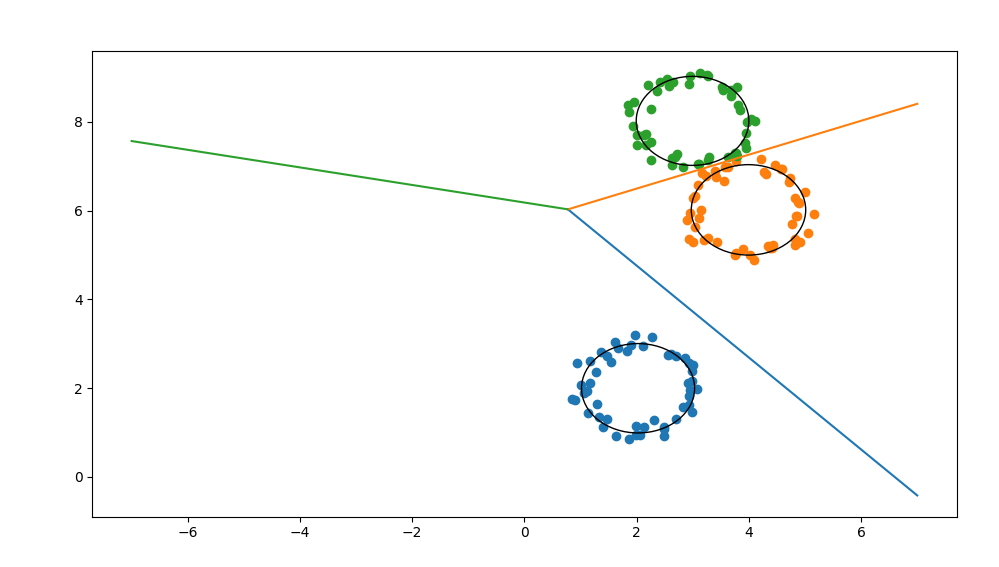
\includegraphics[width=16cm]{hyperplanes.png}
    \caption{The expected output}\label{f:const1}
    \end{center}
\end{figure}

\section{Task 03}
Now we are going to consider trajectory's state prediction $x_k$ each time instance k, in terms of control input sequence $\mathbf{u_k}$ for a given initial condition, i.e., $x_{0|k}$. To estimate the optimal state prediction, an optimal control sequence (or control policy) has to be calculated. Such a control policy can be estimated minimizing the following quadratic cost:

\begin{equation}\label{quadcost}
    J(x_k, \mathbf{u_k}) = \sum_{i=0}^{N-1} \left \| x_{k+i} \right \|_Q^2 + \left \| u_{k+i} \right \|_R^2 + \left \| x_{k+N} \right \|_P^2 
\end{equation} How do you determine the weight matrices: Q, R, and P?
For a linear system, state prediction sequence can be written in a compact sequence as follows:
\begin{equation}
\begin{aligned}
    \mathbf{x_k} = Mx_k + C\mathbf{u_k}, \quad 
    M = \begin{bmatrix}
I\\ 
A\\ 
A^2\\ 
\vdots \\ 
A^N
\end{bmatrix} , \; C = \begin{bmatrix}
0 & 0 & \hdots & 0\\ 
B &  &  & \\ 
AB & B &  & \\ 
 \vdots & \vdots & \ddots & \\ 
A^{N-1}B & A^{N-2}B & \hdots & B 
\end{bmatrix}
\end{aligned}
\end{equation} The defined quadratic cost (\ref{quadcost}) can be written in terms of $\mathbf{x_k}$ and $\mathbf{u_k}$ as 
\begin{equation}\label{unconstriant_1}
    J = \mathbf{x}_k^T\tilde{Q}\mathbf{x_k} + \mathbf{u_k}^T\tilde{R}\mathbf{u_k} = \mathbf{u_k}^TH\mathbf{u_k} + 2x_k^TF^T\mathbf{u_k}+x_k^TGx_k
\end{equation} Can you define the $\tilde{Q}$ and $\tilde{R}$? as well as prove that H, F, and G are given by $C^T\tilde{Q}C + \tilde{R}$, $C^T\tilde{Q}M$, and $M^T\tilde{Q}M$, respectively. Let's say there is no additional constraints are given, \ref{unconstriant_1} has a closed-form solution which can be derived by minimizing the J with respect to $\mathbf{u}$.   Show that $\mathbf{u}^* = -H^{-1}Fx_k$. What can you say about when H is singular (i.e., positive semi-definite rather than positive definite); this implies there are multiple optimal solutions can be exits. Since H and F are constant matrices, $\mathbf{u_k} = Lx_k$, where $L = -H^{-1}F$. 

Now let's try to find out the feedback control law, namely L, considering following second order system with 
\begin{equation} \label{eq1}
   A = \begin{bmatrix}
1.1 & 2\\ 
0 & 0.95
\end{bmatrix}, \quad B = \begin{bmatrix}
0\\ 
0.0787
\end{bmatrix}
\end{equation} for horizon N = 4, you may assume $Q = C^TC$, $R=0.01$, and $P=Q$. 

\section{Task 04}
Here we are interested on terminal constraints set which helps to guarantee the recursive feasibility. In details description about recursive feasibility~\cite{mpc_1, rakovic2016model}.  Let $u_{min}$ and $u_{max}$ be the minimum and maximum values for u, respectively. Let's consider N horizon state prediction as we did before. To ensure u stays within its boundary constraints, i.e.,  $u_{min}$ and $u_{max}$, u always within the $\Omega$ for all $i=0,...,N$

\begin{figure}[H]
    \begin{center}
    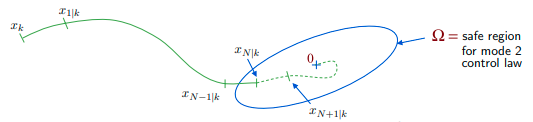
\includegraphics[width=12cm]{terminal.png}
    \caption{The terminal constraint set $\Omega$}\label{f:constraint_set}
    \end{center}
\end{figure}

\begin{equation}
    \Omega = \{ x: u_{min} \leq K(A+BK)^ix \leq u_{max}, \; i=0,...,N\}
\end{equation} where K is the LQ optimal gain. If you do not get whats going on that's all right. Let's get to the the point. Consider the system we examined in (\ref{eq1}) and assume $K = [-1.19 \; -7.88]$. The terminal constraint set can be calculated as follows:
\begin{equation}
    \begin{aligned}
        \Omega_0 = \{x:-1\leq  [-1.19 \; -7.88]x \leq 1 \} \\
        \Omega_1 = \Omega_0 \cap \{x:-1\leq  [-0.5702 \; -4.9572]x \leq 1 \} \\
        \Omega_2 = \Omega_1 \cap \{x:-1\leq  [-0.1621 \; -2.7826]x \leq 1 \} \\
        \vdots
    \end{aligned}
\end{equation}

\begin{figure}[H]
    \begin{center}
    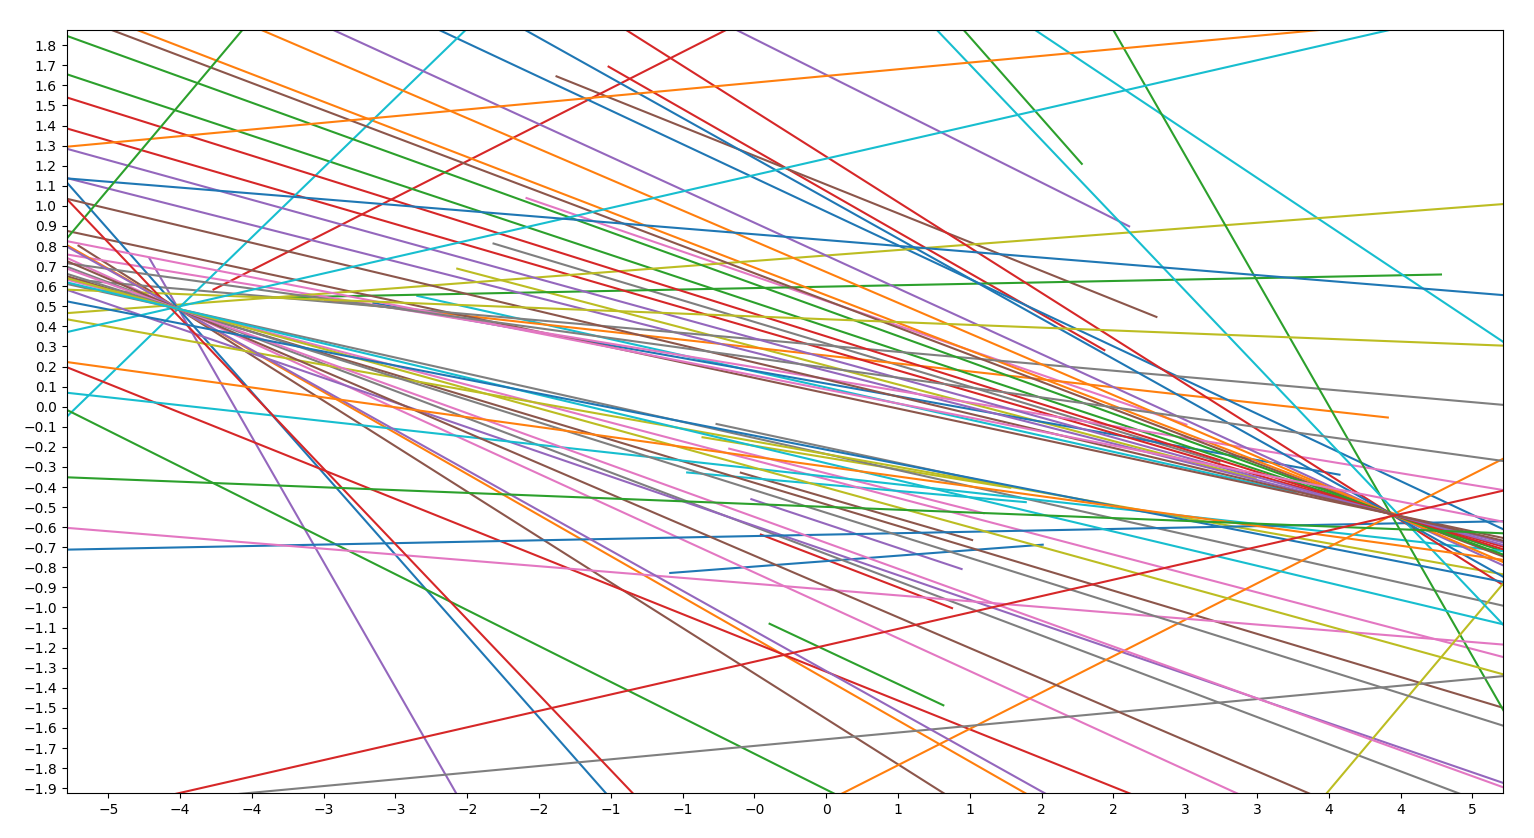
\includegraphics[width=16cm]{mpi_set.png}
    \caption{$\Omega_N = \Omega_{N+1},...,=\Omega_{\infty}$}\label{f:const}
    \end{center}
\end{figure}

If the input u has $n_u$ dimension, how can we estimate $u_{max, j}$ and $u_{min,j}$ for $j=0,..,n_u$? 
\begin{equation}
    \begin{aligned}
         u_{max,j} = \max_x \; K_j(A+BK)^{N+1}x \quad s.t. \; u_{min} \leq K(A+BK)^ix \leq u_{max}, \; i=0,...,N\\
         u_{min,j} = \min_x \; K_j(A+BK)^{N+1}x \quad s.t. \; u_{min} \leq K(A+BK)^ix \leq u_{max},\; i=0,...,N\\
    \end{aligned}
\end{equation} Hence, terminal constraints set finding can be formulated in the following way:

\begin{figure}[H]\label{terminal_set_check}
    \begin{center}
    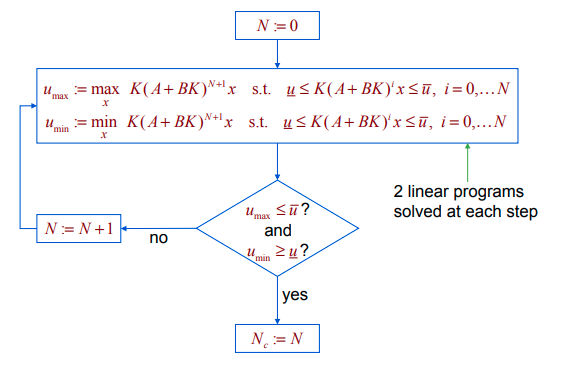
\includegraphics[width=12cm]{fin_t.png}
    \caption{A algorithm for constraint checking~\cite{mpc_1}}\label{f:fin_t}
    \end{center}
\end{figure}

\begin{figure}[H]
    \begin{center}
    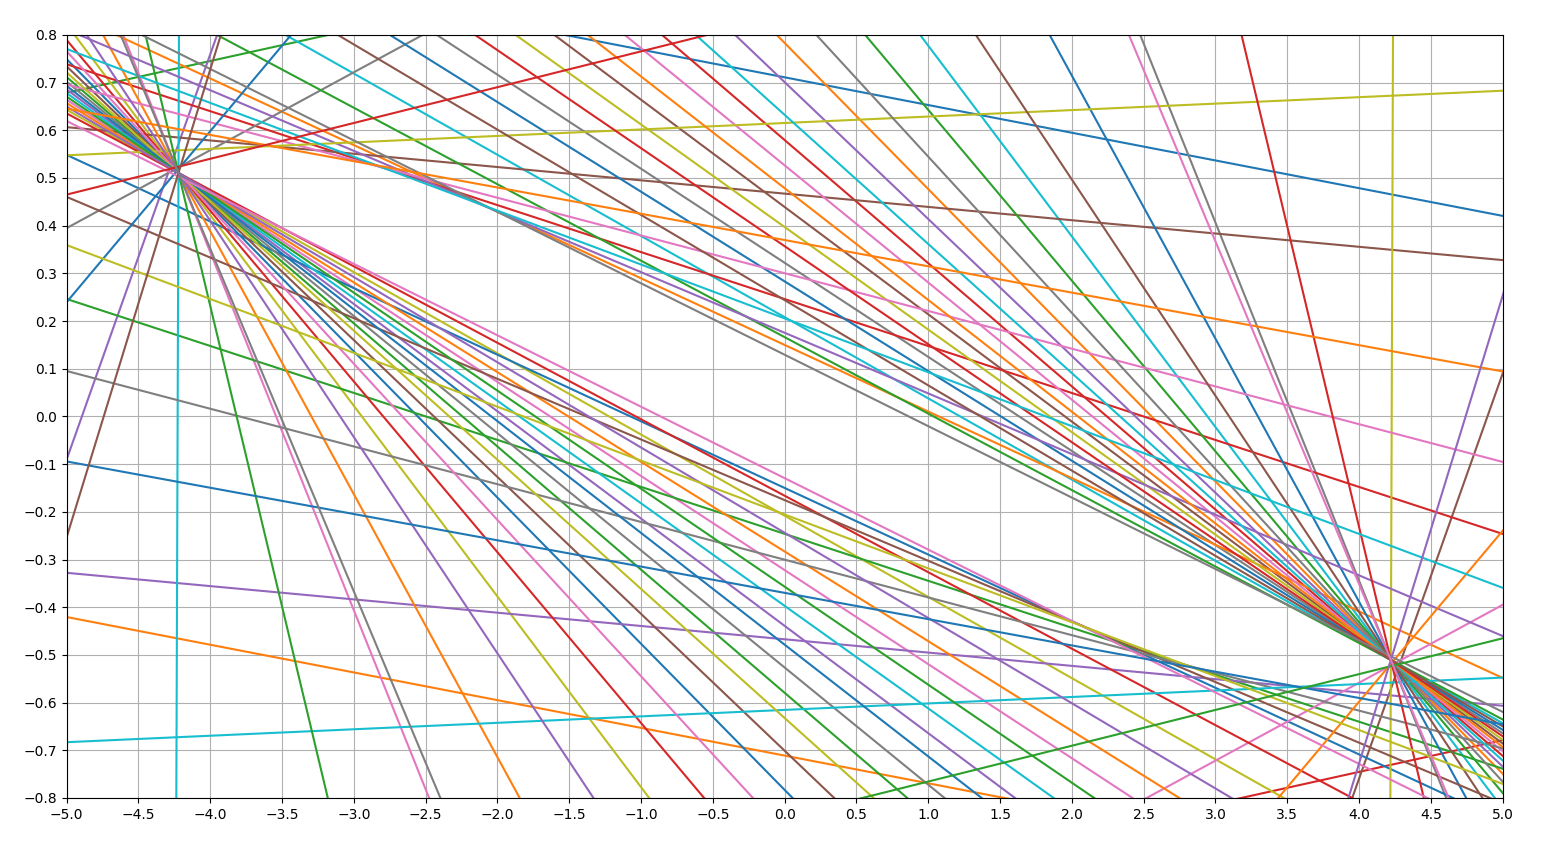
\includegraphics[width=12cm]{final_set.png}
    \caption{The terminal set after applying algorithm \ref{f:fin_t} }\label{f:final_set}
    \end{center}
\end{figure}

\begin{enumerate}
    \item Use linprog for formulate Algorithm.\ref{f:fin_t}, you may use following function for plotting the linear inequalities
    
    


\begin{minted}
[frame=lines, framesep=2mm, baselinestretch=1.2,]
{python}

import matplotlib.pyplot as plt
import numpy as np
from scipy.optimize import linprog

def plot_line(slope, intercept):
    axes = plt.gca()
    x_vals = np.array(axes.get_xlim())
    y_vals = intercept + slope * x_vals
    start, end = axes.get_xlim()
    axes.xaxis.set_ticks(np.arange(start, end, 0.5))
    start, end = axes.get_ylim()
    axes.yaxis.set_ticks(np.arange(start, end, 0.1))
    plt.plot(x_vals, y_vals, '-')

plt.ylim((-0.8, 0.8))
plt.xlim((-5,5))

\end{minted}
\end{enumerate}


\section{Task 05}
Assume a system dynamics is described in terms of LTI (linear time invariant) state-space model 
\begin{equation} \label{dynamics}
   \begin{aligned}
    x_{k+1} = Ax_k + Bu_k \\
    y_k = Cx_k,
   \end{aligned}
\end{equation} where $x_k \in \mathbb{R}^{n_x}$, $u_k \in \mathbb{R}^{n_u}$, and $y_k \in \mathbb{R}^{n_y}$. Such control system is assumed be enforced by a set of linear constraints, i.e., may involve both state and inputs. In general, those can be expressed as 
\begin{equation}\label{constraints}
    \begin{aligned}
        Fx + Gu \leq 1,
    \end{aligned}
\end{equation} where $F \in \mathbb{R}^{n_c\times n_x}$ and $ G \in \mathbb{R}^{n_c\times n_u}$. 

\begin{theorem}
     The MPI (Maximum Positive Invariant) set for the system with dynamics (\ref{dynamics}) and the system constraints set (\ref{constraints}) can be defined as:
     \begin{equation}
         X^{MPI} \doteq \{ x: (F+GK)\Phi^ix\leq1, \; i=0,...,v\} ,
     \end{equation}
\end{theorem} where v is the smallest positive integer such that $(F+GK)\Phi^{v+1}x \leq 1$, $\forall x$ satisfying $(F+GK)\Phi^ix \leq 1, \; i=0,...,v$. $\Phi$ is determined as $A + B\cdot K$. The value of v can be computed by solving following LPs, namely 

\begin{equation}\label{max_volume}
\begin{aligned}
\max_{x} \quad & (F+GK)_j\Phi^{n+1}x\\
\textrm{s.t.} \quad & (F+GK)\Phi^ix \leq 1, \; i=0,...,n
\end{aligned}
\end{equation} for $j=1,...,n_c$, n=1,...,v, where $(F+GK)_j$ denotes the jth row of F+GK. 

Now considering following second order system with 
\begin{equation} \label{eq1}
   A = \begin{bmatrix}
1.1 & 2\\ 
0 & 0.95
\end{bmatrix}, \quad B = \begin{bmatrix}
0\\ 
0.0787
\end{bmatrix}
\end{equation} whose constraints are given by $-1\leq x/8 \leq 1$ and $ \; -1 \leq u \leq 1$. With listed constraints we can define the F and G as follows: 
\begin{equation}
    F = \begin{bmatrix}
0 & 1/8\\ 
1/8 & 0\\ 
0 & -1/8\\ 
-1/8 & 0\\ 
 0&0 \\ 
0 & 0
\end{bmatrix}, \; G = \begin{bmatrix}
0\\ 
0\\ 
0\\ 
0\\ 
1\\ 
-1
\end{bmatrix}
\end{equation}

Calculate the MPI set for this system where assume value of v some value in between 5 to 20. The following helper functions may help you.

\begin{minted}
[frame=lines, framesep=2mm, baselinestretch=1.2,]
{python}
import matplotlib.pyplot as plt
import numpy as np
from scipy.optimize import linprog

def plot_line(slope, intercept, range_xval=(-8, 8)):
    axes = plt.gca()
    x_vals = np.array(axes.get_xlim())
    y_vals = intercept + slope * x_vals
    start, end = axes.get_xlim()
    axes.xaxis.set_ticks(np.arange(start, end, 0.5))
    start, end = axes.get_ylim()
    axes.yaxis.set_ticks(np.arange(start, end, 0.1))
    plt.plot(x_vals, y_vals, '-')
    


\end{minted}

\begin{minted}
[frame=lines, framesep=2mm, baselinestretch=1.2,]
{python}
bnd = [(-8, 8), (-8, 8)]
opt = linprog(c=obj, A_ub=lhs_ineq, b_ub=rhs_ineq, bounds=bnd)
\end{minted}

The expected output something similar to this:
\begin{figure}[H]
    \begin{center}
    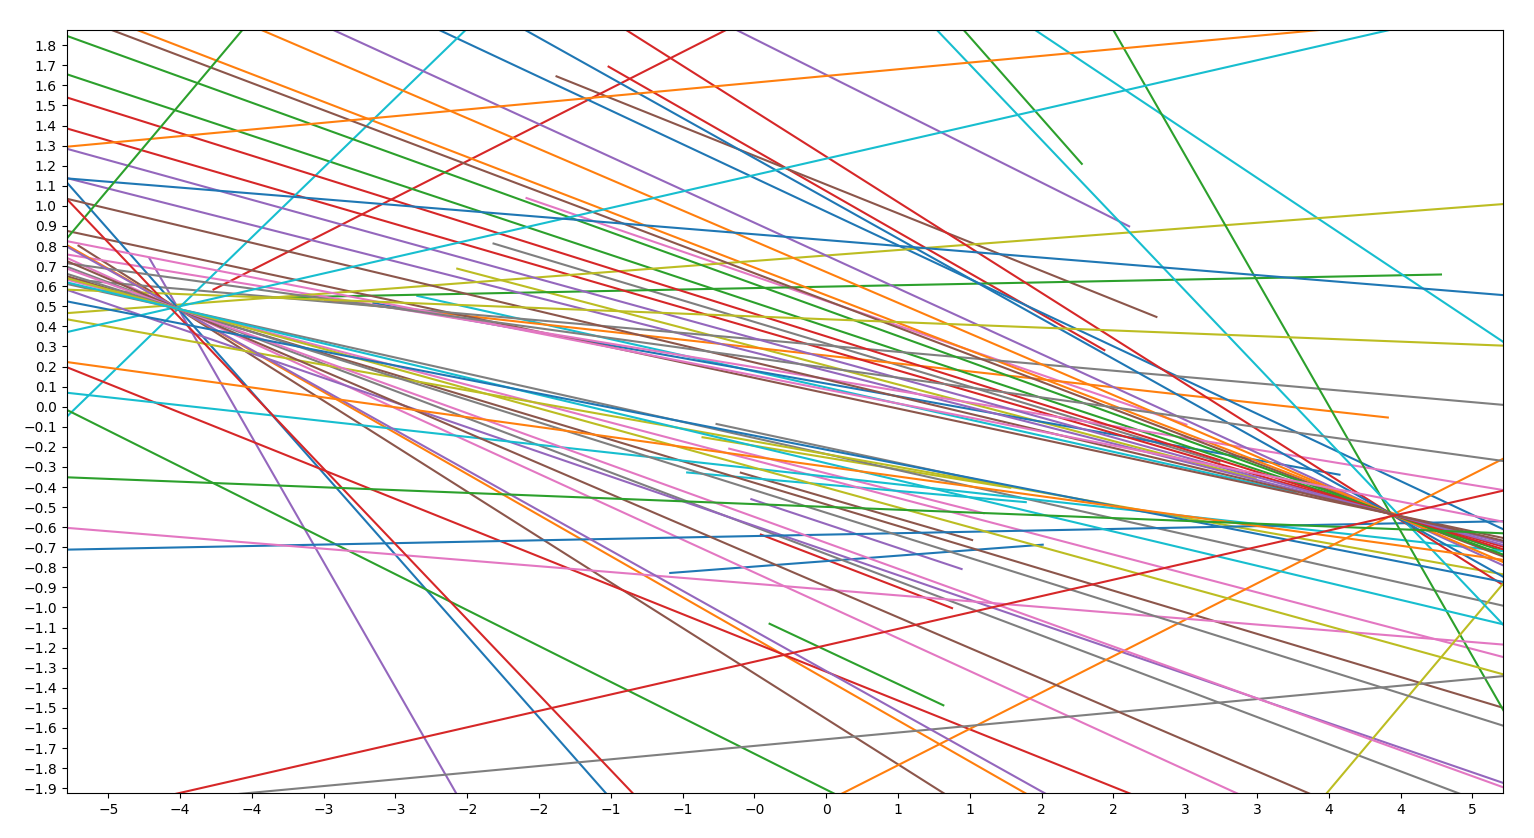
\includegraphics[width=16cm]{mpi_set.png}
    \caption{}
    \end{center}
\end{figure}



\printbibliography
\end{document}